% PKUMpLtX --- A LaTeX document class for 'Modern Physics Laboratory' in PKU based on `revtex4-2`
%
% Please read `README.md' and the template file before using
% 需要确保 font 选项指定的字体已安装! 具体参见 `README.md' 的说明.
\documentclass[font=default]{mpltx}

% 以下至 \begin{document} 都仅是本文件为了方便额外定义的命令, 写报告时不需要.
\hypersetup{colorlinks=true}% 超链接带颜色
\usepackage{xcolor}
\usepackage{tcolorbox}

\newtcbox{\buttombox}[1][red]
  {on line, arc = 3pt, outer arc = 3pt,
    colback = #1!10!white, colframe = #1!50!black,
    boxsep = 0pt, left = 2pt, right = 2pt, top = 1pt, bottom = 1pt,
    boxrule = 1pt}

\newcommand{\note}[1]{{\color{gray}#1}}
\NewDocumentCommand{\pkg}{s o m}{%
    \IfBooleanF{#1}{%
        \IfNoValueTF{#2}%
            {\href{https://www.ctan.org/pkg/#3}}%
            {\href{https://www.ctan.org/pkg/#2}}%
    }%
    {\textsf{#3}}%
}
\newcommand*\cs[1]{\texttt{\textbackslash #1}}
\newcommand*\env[1]{\textit{\texttt{#1}}}
\newcommand*\code[1]{\texttt{#1}}
\newcommand*\file[1]{\textbf{\texttt{#1}}}
\makeatletter
\newcommand\releasedate{%
    \href{https://github.com/CastleStar14654/PKUMpLtX/releases/tag/\mpltx@fileversion}%
        {\mpltx@filedate, \mpltx@fileversion}}
\makeatother
% 以上是本文件为了方便额外定义的命令, 写报告时不需要.

\begin{document}

\title{半导体激光器激光谱线特性测量} % 切合报告内容, 简短明确, 可以不同于讲义
\author{罗俊熙} % 这里 \emailphone 一定要紧跟在 \author 后方
\emailphone{see.looooo@stu.pku.edu.cn}{(86)13611162432}
% 如果改用 \email 则仅需要邮箱参数
\affiliation{北京大学物理学院\quad 学号: 2000012508}
% % 可以使用 \zhdate 自动生成中文日期, 如
% \date{\zhdate{2020/12/1}}
% % 也可使用 babel 的 \localedate, 如
% \date{\localedate{2020}{12}{1}}
% % 两者均会输出 `2020 年 12 月 1 日'
% 下面的 \date 的参数是为了自动输出正确版本号, 正式报告请替换为上面的两种 \date 之一
\date{\localedate{2023}{03}{18}}
\begin{abstract}
	半导体激光器是一种将电能转换为光能的电光转换器件,它是由半导体材料制成的。
	通常采用PN结或P型和N型掺杂区的结构,当外加电压时,
	电子和空穴在掺杂区结合并释放出能量,这些能量被放大后转化为激光光束输出。
	本次实验使用半导体激光器产生的激光,通过接后屏射后进入 Fabry-Perot 标准具产生干涉条纹,用以测量半导体激光器的激光谱线宽。
\end{abstract}
\keywords{半导体激光器、激光谱线特性、Fabry-Perot 标准具}

\maketitle

\section{引言}
半导体激光器,又称激光二极管,是使用半导体材料作为工作物质的一种激光器,
是目前最实用、最重要的激光器之一。它具有高效率、小体积、轻便、价格低等优点,
在激光通信、光存储、光陀螺、激光打印、测距和雷达等领域得到了广泛应用。
其工作原理是通过一定的激励方式,在半导体物质的能带(导带与价带)之间,
或者半导体物质的能带与杂质(受主或施主)能级之间,实现非平衡载流子的粒子数反转。
当处于粒子数反转状态的大量电子与空穴复合时,就会产生受激发射作用,从而产生激光。
本实验利用F-P标准具产生干涉条纹,用以测量半导体激光器的激光谱线特性,
包括激光谱线宽度$\Delta\lambda$等参数。

\section{实验目的}
\begin{enumerate}
	\item 本实验旨在掌握使用单色仪和F-P标准具测量半导体激光器激光谱线特性的方法。
	      具体而言,我们将学习如何使用单色仪获取半导体激光器的激光光谱,
	      并利用F-P标准具产生干涉条纹,通过对条纹的分析计算出激光谱线的参数,
	      例如激光谱线宽度等。
	\item 通过CCD-计算机图像采集系统获取的图像文件,
	      我们可以使用图像分析方法来计算出与物理参数相关的参数值。在本实验中,
	      我们将学习如何使用图像分析技术,通过对图像文件的处理和分析,
	      获取与半导体激光器激光谱线特性相关的物理参数,例如激光谱线的峰值强度、波长等。
\end{enumerate}

\section{理论}\label{sec:theory}
\subsection{半导体作为光的增益介质}
增益介质是能够让光信号得到放大的一种物质。这种放大效应通常是由于增益介质内部的电
子在某些能级之间实现粒子数反转所导致的。在粒子数反转状态下,电子在两个能级之间跃
迁,从高能级到低能级跃迁时放出一定频率的光。通过这种受激辐射作用,光信号得以放大
。因此,增益介质也被称为激活介质。在半导体材料中,有多种不同的发光机制,如激自发
光和杂质发光等。其中,最主要的发光机制是电子-空穴复合发光,即从导带到价带的跃迁。\par

在这种跃迁机制中,电子跃迁的上、下能级分别是半导体的导带和价带。对应的能量为$E_C$和$E_V$在半导体中,通过
掺入施主或受主杂质,可以使材料中存在更多的自由电子或空穴,分别形成n型和p型半导体
。同时,制作一侧为n型区一侧为p型区的半导体,形成 p-n 结。如\autoref{fig:1}所示,当未加电场时,
p型区和n型区的费米能级$E_F$在同一水平处于热平衡状态。此时,p-n 结区域存在能量势垒$E_g=E_C-E_V$,
使得n型区的电子不能进入p型区,反之亦然。\par

\begin{figure}
	\centering
	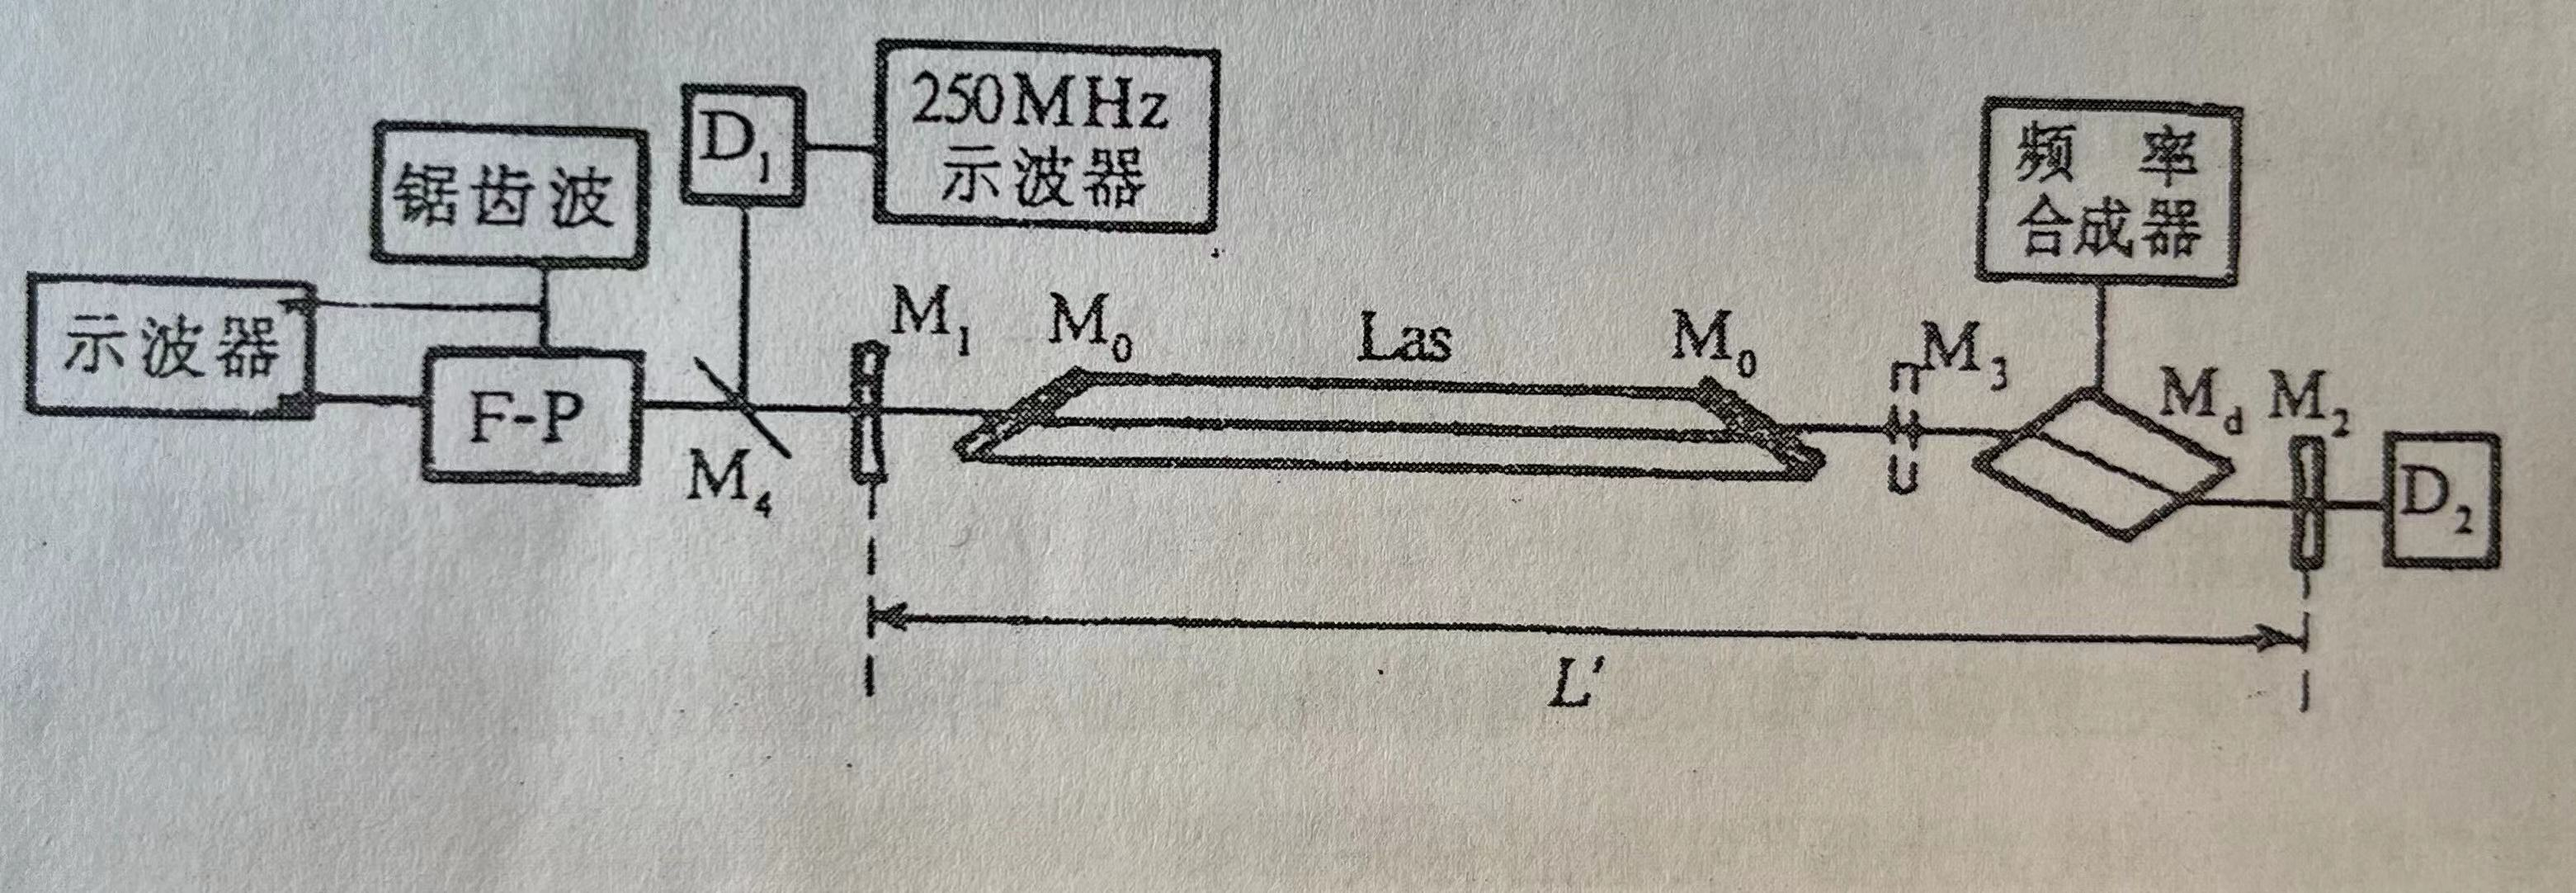
\includegraphics[width=0.85\linewidth]{fig/1.jpg}
	\caption{未加偏置电压时半导体激光器的能带。\cite{laser}}
	\label{fig:1}
\end{figure}

因此,在n型区,电子是多数载流子,空穴是少数载流子,而在p型区,空穴是多数载流子,电子是少数载流子。\par

产生受激辐射的条件是结区的导带底部和价带顶部形成粒子数反转分布。当在 p-n 结上加正向
电压V时,势垒降低,外加的电源会往n型区注入电子,往p型区注入空穴,导致半导体处于非
平衡态,形成结区两个费米分布$f_e(E)$和$f_h(E)$两个费米能级,即准费米能级$E_{F_n}$和$E_{F_p}$,如
\autoref{fig:2}所示。此时:
\begin{enumerate}
	\item n型区的电子通过 p-n 结向p区运动。
	\item p型区的空穴通过 p-n 结向n区运动。
\end{enumerate}
在 p-n 结区(激活区/有源层)处会产生粒子数反转,电子和空穴会以光子形式释放出能量。这就是半导体作为增益介质,在电流注入时的电子-空穴复合发光机理。\par

利用谐振腔可以将以上发光过程产生的光场限制在几个模式中,使能量集中光场增强,并使增
益大于损耗,则可产生受激辐射,从而实现半导体激光器的工作。半导体激光器产生激光震荡
和受激发射的必要条件是电子和空穴的分布不处于热平衡状态,而是粒子数反转状态。通过电
流注入或光激发的方式,可以产生非热平衡的分布,使得:

$E_{F_n} - E_{F_p} > h_\nu > E_g$

此时系统可以对光进行放大,成为具有增益的工作介质。

\section{实验装置及流程}
\subsection{实验装置}
实验装置由半导体激光器、F-P 干涉仪、屏幕所组成。
\begin{enumerate}
	\item 半导体激光器:发射红色激光的小功率半导体激光器,被置于调节架上便于调整光束方向;
	\item F-P 标准具:法布里-珀罗标准具,用于测量半导体激光器的线宽;
	\item 计算机系统:利用 F-P 标准具的干涉图像分析谱线的线宽。
\end{enumerate}

\subsection{实验过程及结果}
\subsubsection{半导体激光波长的标定}

实验略过对半导体激光波长的标定,给出半导体激光波长为\qty{632.8}{\nm}\par

\subsubsection{半导体激光谱线宽度的测量}
利用 F-P 标准具测量线宽,其产生干涉极大的条件为:

$$2nl\cos{\theta} = k\lambda$$

其中,$n$ 为折射率(空气间隔的标准具 $n = 1$),$l = \qty{4.25}{\mm}$ 为间隔圈长度,$\theta$为光线的入射角,$k$ 为干涉序。

首先,我们利用半导体激光器、F-P 标准具(有可使激光漫散射的毛玻璃)和接收屏搭建光路(如\autoref{fig:3}所示),直到显示出干涉条纹,并调整标准具上的三个微调螺丝。使用眼睛观察干涉花纹,若花纹随眼睛上下左右移动时有收缩或扩张(中心花纹吞吐)变化,则调整微调螺丝,直到花纹稳定不随观察方向的移动变化。

我们用焦距为$f$的透镜把干涉环成像在焦平面上,环的直径用$D$表示,中心附近几序干涉环的入射角很小,可近似为:

$$\cos{\theta} \approx 1 − \frac{\theta^2}{2}, \theta \approx \frac{D}{2f}$$

因此得到:

$$2l\left(1-\frac{1}{8}\left(\frac{D}{f}\right)^2\right)W=k\lambda$$

此式可以用干涉花纹宽度测量光谱线宽度。设与 $k$ 序的干涉环宽度 $\Delta\lambda$ 对应的内外直径 $D_{k,i}$ 和 $D_{k,o}$,中心花纹附近的干涉环的 $k$ 值用中心花纹 $k =2\frac{l}{\lambda}$ 代替,得到:

\begin{equation}\label{eq:1}
	\Delta\lambda = \frac{\lambda}{2f^2}(D^2_{k,i}-D^2_{k,o})
\end{equation}

由于我们没有手机摄像头的焦距 $f$,而且像并不是直接成在手机 CCD 上,不能利用上式计算谱线宽度 $\Delta\lambda$。利用式1,对$k = j$及 $k = j + 1$ 的干涉条纹,我们可以得到:

$$\frac{l}{4f^2}(D^2_{k=j}-D^2_{k=j+1})=\lambda$$

此时代入\autoref{eq:1},我们得到:
\begin{equation}\label{eq:2}
	\Delta \lambda = \frac{\lambda^2}{2l}\frac{(D^2_{k=j,i}-D^2_{k=j,o})}{(D^2_{k=j}-D^2_{k=j+1})}
\end{equation}
利用上式就可以不知道焦距$f$的情况下求得谱线宽度$\Delta\lambda$了。
\subsubsection{分析干涉图像}
我们利用程序得到条纹内外径如\autoref{fig:5}显示,结合利用上式得到的数据如\autoref{tab:1}所示。其所得谱线宽度 $\Delta\lambda$ 的估计为:
$$\Delta\lambda=\qty{1.0\pm0.2}{\pm}$$

\section{结论}
\textbf{本次实验使用半导体激光器产生的激光,通过接后屏射后进入 Fabry-Perot 标准具产生干涉条纹,用以测量半导体激光器的激光谱线宽。
	通过对干涉条纹的分析,我们得出了半导体激光器的激光谱线宽的值为 $\qty{123}{\pm}$。}

% bibliography 的参数是你的 *.bib 文件去掉后缀名后的部分
\bibliography{bibli}

\clearpage % 附录前另起一页
\appendix % 附录开始
\section{思考题}\label{app:exercise}
\subsection{为甚么实验失败?}
\subsection{锁模用的声光调制哭能用行波的方式工作吗?为甚么?}
\subsection{为甚么要把声光调制器安放在尽量靠近谐振腔反射镜的一端?}
\subsection{请设计一个准确测量锁模脉宽的方案。}

\end{document}
